% Created by tikzDevice version 0.12.3 on 2019-09-30 11:20:19
% !TEX encoding = UTF-8 Unicode
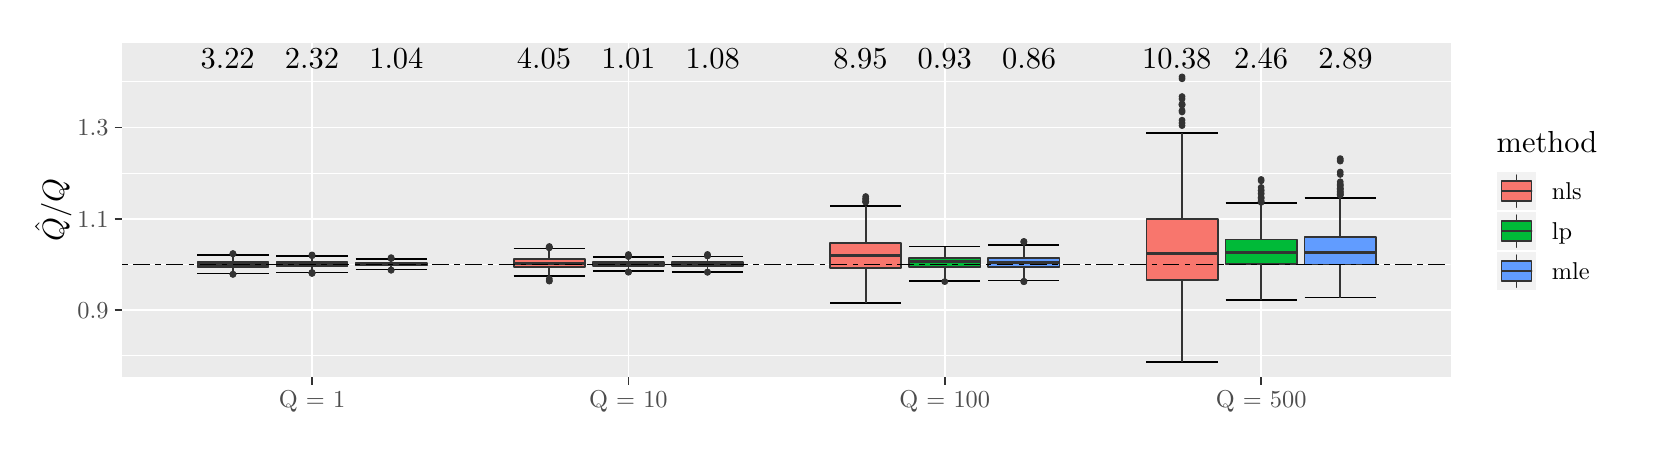
\begin{tikzpicture}[x=1pt,y=1pt]
\definecolor{fillColor}{RGB}{255,255,255}
\path[use as bounding box,fill=fillColor,fill opacity=0.00] (0,0) rectangle (578.16,144.54);
\begin{scope}
\path[clip] (  0.00,  0.00) rectangle (578.16,144.54);
\definecolor{drawColor}{RGB}{255,255,255}
\definecolor{fillColor}{RGB}{255,255,255}

\path[draw=drawColor,line width= 0.6pt,line join=round,line cap=round,fill=fillColor] (  0.00,  0.00) rectangle (578.16,144.54);
\end{scope}
\begin{scope}
\path[clip] ( 34.16, 18.22) rectangle (514.31,139.04);
\definecolor{fillColor}{gray}{0.92}

\path[fill=fillColor] ( 34.16, 18.22) rectangle (514.31,139.04);
\definecolor{drawColor}{RGB}{255,255,255}

\path[draw=drawColor,line width= 0.3pt,line join=round] ( 34.16, 26.06) --
	(514.31, 26.06);

\path[draw=drawColor,line width= 0.3pt,line join=round] ( 34.16, 59.02) --
	(514.31, 59.02);

\path[draw=drawColor,line width= 0.3pt,line join=round] ( 34.16, 91.98) --
	(514.31, 91.98);

\path[draw=drawColor,line width= 0.3pt,line join=round] ( 34.16,124.94) --
	(514.31,124.94);

\path[draw=drawColor,line width= 0.6pt,line join=round] ( 34.16, 42.54) --
	(514.31, 42.54);

\path[draw=drawColor,line width= 0.6pt,line join=round] ( 34.16, 75.50) --
	(514.31, 75.50);

\path[draw=drawColor,line width= 0.6pt,line join=round] ( 34.16,108.46) --
	(514.31,108.46);

\path[draw=drawColor,line width= 0.6pt,line join=round] (102.75, 18.22) --
	(102.75,139.04);

\path[draw=drawColor,line width= 0.6pt,line join=round] (217.07, 18.22) --
	(217.07,139.04);

\path[draw=drawColor,line width= 0.6pt,line join=round] (331.39, 18.22) --
	(331.39,139.04);

\path[draw=drawColor,line width= 0.6pt,line join=round] (445.71, 18.22) --
	(445.71,139.04);
\definecolor{drawColor}{RGB}{0,0,0}

\path[draw=drawColor,line width= 0.6pt,line join=round] ( 61.31, 62.51) --
	( 87.03, 62.51);

\path[draw=drawColor,line width= 0.6pt,line join=round] ( 74.17, 62.51) --
	( 74.17, 55.75);

\path[draw=drawColor,line width= 0.6pt,line join=round] ( 61.31, 55.75) --
	( 87.03, 55.75);

\path[draw=drawColor,line width= 0.6pt,line join=round] ( 89.89, 61.97) --
	(115.61, 61.97);

\path[draw=drawColor,line width= 0.6pt,line join=round] (102.75, 61.97) --
	(102.75, 56.12);

\path[draw=drawColor,line width= 0.6pt,line join=round] ( 89.89, 56.12) --
	(115.61, 56.12);

\path[draw=drawColor,line width= 0.6pt,line join=round] (118.47, 60.94) --
	(144.19, 60.94);

\path[draw=drawColor,line width= 0.6pt,line join=round] (131.33, 60.94) --
	(131.33, 57.10);

\path[draw=drawColor,line width= 0.6pt,line join=round] (118.47, 57.10) --
	(144.19, 57.10);

\path[draw=drawColor,line width= 0.6pt,line join=round] (175.63, 64.79) --
	(201.35, 64.79);

\path[draw=drawColor,line width= 0.6pt,line join=round] (188.49, 64.79) --
	(188.49, 54.70);

\path[draw=drawColor,line width= 0.6pt,line join=round] (175.63, 54.70) --
	(201.35, 54.70);

\path[draw=drawColor,line width= 0.6pt,line join=round] (204.21, 61.71) --
	(229.93, 61.71);

\path[draw=drawColor,line width= 0.6pt,line join=round] (217.07, 61.71) --
	(217.07, 56.61);

\path[draw=drawColor,line width= 0.6pt,line join=round] (204.21, 56.61) --
	(229.93, 56.61);

\path[draw=drawColor,line width= 0.6pt,line join=round] (232.79, 61.90) --
	(258.51, 61.90);

\path[draw=drawColor,line width= 0.6pt,line join=round] (245.65, 61.90) --
	(245.65, 56.37);

\path[draw=drawColor,line width= 0.6pt,line join=round] (232.79, 56.37) --
	(258.51, 56.37);

\path[draw=drawColor,line width= 0.6pt,line join=round] (289.95, 80.09) --
	(315.67, 80.09);

\path[draw=drawColor,line width= 0.6pt,line join=round] (302.81, 80.09) --
	(302.81, 45.07);

\path[draw=drawColor,line width= 0.6pt,line join=round] (289.95, 45.07) --
	(315.67, 45.07);

\path[draw=drawColor,line width= 0.6pt,line join=round] (318.53, 65.42) --
	(344.25, 65.42);

\path[draw=drawColor,line width= 0.6pt,line join=round] (331.39, 65.42) --
	(331.39, 52.97);

\path[draw=drawColor,line width= 0.6pt,line join=round] (318.53, 52.97) --
	(344.25, 52.97);

\path[draw=drawColor,line width= 0.6pt,line join=round] (347.11, 65.96) --
	(372.83, 65.96);

\path[draw=drawColor,line width= 0.6pt,line join=round] (359.97, 65.96) --
	(359.97, 53.24);

\path[draw=drawColor,line width= 0.6pt,line join=round] (347.11, 53.24) --
	(372.83, 53.24);

\path[draw=drawColor,line width= 0.6pt,line join=round] (404.27,106.49) --
	(430.00,106.49);

\path[draw=drawColor,line width= 0.6pt,line join=round] (417.13,106.49) --
	(417.13, 23.71);

\path[draw=drawColor,line width= 0.6pt,line join=round] (404.27, 23.71) --
	(430.00, 23.71);

\path[draw=drawColor,line width= 0.6pt,line join=round] (432.85, 81.29) --
	(458.58, 81.29);

\path[draw=drawColor,line width= 0.6pt,line join=round] (445.71, 81.29) --
	(445.71, 46.19);

\path[draw=drawColor,line width= 0.6pt,line join=round] (432.85, 46.19) --
	(458.58, 46.19);

\path[draw=drawColor,line width= 0.6pt,line join=round] (461.43, 82.95) --
	(487.16, 82.95);

\path[draw=drawColor,line width= 0.6pt,line join=round] (474.29, 82.95) --
	(474.29, 46.99);

\path[draw=drawColor,line width= 0.6pt,line join=round] (461.43, 46.99) --
	(487.16, 46.99);
\definecolor{drawColor}{gray}{0.20}
\definecolor{fillColor}{gray}{0.20}

\path[draw=drawColor,line width= 0.4pt,line join=round,line cap=round,fill=fillColor] ( 74.17, 62.92) circle (  1.02);

\path[draw=drawColor,line width= 0.4pt,line join=round,line cap=round,fill=fillColor] ( 74.17, 55.43) circle (  1.02);

\path[draw=drawColor,line width= 0.4pt,line join=round,line cap=round,fill=fillColor] ( 74.17, 55.42) circle (  1.02);

\path[draw=drawColor,line width= 0.4pt,line join=round,line cap=round,fill=fillColor] ( 74.17, 62.80) circle (  1.02);

\path[draw=drawColor,line width= 0.6pt,line join=round] ( 74.17, 59.88) -- ( 74.17, 62.51);

\path[draw=drawColor,line width= 0.6pt,line join=round] ( 74.17, 58.12) -- ( 74.17, 55.75);
\definecolor{fillColor}{RGB}{248,118,109}

\path[draw=drawColor,line width= 0.6pt,line join=round,line cap=round,fill=fillColor] ( 61.31, 59.88) --
	( 61.31, 58.12) --
	( 87.03, 58.12) --
	( 87.03, 59.88) --
	( 61.31, 59.88) --
	cycle;

\path[draw=drawColor,line width= 1.1pt,line join=round] ( 61.31, 58.96) -- ( 87.03, 58.96);
\definecolor{fillColor}{gray}{0.20}

\path[draw=drawColor,line width= 0.4pt,line join=round,line cap=round,fill=fillColor] (102.75, 56.06) circle (  1.02);

\path[draw=drawColor,line width= 0.4pt,line join=round,line cap=round,fill=fillColor] (102.75, 55.96) circle (  1.02);

\path[draw=drawColor,line width= 0.4pt,line join=round,line cap=round,fill=fillColor] (102.75, 62.12) circle (  1.02);

\path[draw=drawColor,line width= 0.4pt,line join=round,line cap=round,fill=fillColor] (102.75, 62.43) circle (  1.02);

\path[draw=drawColor,line width= 0.4pt,line join=round,line cap=round,fill=fillColor] (102.75, 55.72) circle (  1.02);

\path[draw=drawColor,line width= 0.4pt,line join=round,line cap=round,fill=fillColor] (102.75, 55.92) circle (  1.02);

\path[draw=drawColor,line width= 0.6pt,line join=round] (102.75, 59.76) -- (102.75, 61.97);

\path[draw=drawColor,line width= 0.6pt,line join=round] (102.75, 58.29) -- (102.75, 56.12);
\definecolor{fillColor}{RGB}{0,186,56}

\path[draw=drawColor,line width= 0.6pt,line join=round,line cap=round,fill=fillColor] ( 89.89, 59.76) --
	( 89.89, 58.29) --
	(115.61, 58.29) --
	(115.61, 59.76) --
	( 89.89, 59.76) --
	cycle;

\path[draw=drawColor,line width= 1.1pt,line join=round] ( 89.89, 59.02) -- (115.61, 59.02);
\definecolor{fillColor}{gray}{0.20}

\path[draw=drawColor,line width= 0.4pt,line join=round,line cap=round,fill=fillColor] (131.33, 56.97) circle (  1.02);

\path[draw=drawColor,line width= 0.4pt,line join=round,line cap=round,fill=fillColor] (131.33, 61.45) circle (  1.02);

\path[draw=drawColor,line width= 0.4pt,line join=round,line cap=round,fill=fillColor] (131.33, 61.13) circle (  1.02);

\path[draw=drawColor,line width= 0.4pt,line join=round,line cap=round,fill=fillColor] (131.33, 61.17) circle (  1.02);

\path[draw=drawColor,line width= 0.4pt,line join=round,line cap=round,fill=fillColor] (131.33, 56.90) circle (  1.02);

\path[draw=drawColor,line width= 0.6pt,line join=round] (131.33, 59.52) -- (131.33, 60.94);

\path[draw=drawColor,line width= 0.6pt,line join=round] (131.33, 58.54) -- (131.33, 57.10);
\definecolor{fillColor}{RGB}{97,156,255}

\path[draw=drawColor,line width= 0.6pt,line join=round,line cap=round,fill=fillColor] (118.47, 59.52) --
	(118.47, 58.54) --
	(144.19, 58.54) --
	(144.19, 59.52) --
	(118.47, 59.52) --
	cycle;

\path[draw=drawColor,line width= 1.1pt,line join=round] (118.47, 59.02) -- (144.19, 59.02);
\definecolor{fillColor}{gray}{0.20}

\path[draw=drawColor,line width= 0.4pt,line join=round,line cap=round,fill=fillColor] (188.49, 52.98) circle (  1.02);

\path[draw=drawColor,line width= 0.4pt,line join=round,line cap=round,fill=fillColor] (188.49, 65.06) circle (  1.02);

\path[draw=drawColor,line width= 0.4pt,line join=round,line cap=round,fill=fillColor] (188.49, 65.18) circle (  1.02);

\path[draw=drawColor,line width= 0.4pt,line join=round,line cap=round,fill=fillColor] (188.49, 53.04) circle (  1.02);

\path[draw=drawColor,line width= 0.4pt,line join=round,line cap=round,fill=fillColor] (188.49, 53.80) circle (  1.02);

\path[draw=drawColor,line width= 0.4pt,line join=round,line cap=round,fill=fillColor] (188.49, 65.47) circle (  1.02);

\path[draw=drawColor,line width= 0.4pt,line join=round,line cap=round,fill=fillColor] (188.49, 65.02) circle (  1.02);

\path[draw=drawColor,line width= 0.6pt,line join=round] (188.49, 60.84) -- (188.49, 64.79);

\path[draw=drawColor,line width= 0.6pt,line join=round] (188.49, 58.14) -- (188.49, 54.70);
\definecolor{fillColor}{RGB}{248,118,109}

\path[draw=drawColor,line width= 0.6pt,line join=round,line cap=round,fill=fillColor] (175.63, 60.84) --
	(175.63, 58.14) --
	(201.35, 58.14) --
	(201.35, 60.84) --
	(175.63, 60.84) --
	cycle;

\path[draw=drawColor,line width= 1.1pt,line join=round] (175.63, 59.47) -- (201.35, 59.47);
\definecolor{fillColor}{gray}{0.20}

\path[draw=drawColor,line width= 0.4pt,line join=round,line cap=round,fill=fillColor] (217.07, 56.30) circle (  1.02);

\path[draw=drawColor,line width= 0.4pt,line join=round,line cap=round,fill=fillColor] (217.07, 62.03) circle (  1.02);

\path[draw=drawColor,line width= 0.4pt,line join=round,line cap=round,fill=fillColor] (217.07, 56.20) circle (  1.02);

\path[draw=drawColor,line width= 0.4pt,line join=round,line cap=round,fill=fillColor] (217.07, 62.07) circle (  1.02);

\path[draw=drawColor,line width= 0.4pt,line join=round,line cap=round,fill=fillColor] (217.07, 56.24) circle (  1.02);

\path[draw=drawColor,line width= 0.4pt,line join=round,line cap=round,fill=fillColor] (217.07, 62.00) circle (  1.02);

\path[draw=drawColor,line width= 0.4pt,line join=round,line cap=round,fill=fillColor] (217.07, 62.56) circle (  1.02);

\path[draw=drawColor,line width= 0.4pt,line join=round,line cap=round,fill=fillColor] (217.07, 61.85) circle (  1.02);

\path[draw=drawColor,line width= 0.4pt,line join=round,line cap=round,fill=fillColor] (217.07, 61.98) circle (  1.02);

\path[draw=drawColor,line width= 0.4pt,line join=round,line cap=round,fill=fillColor] (217.07, 62.08) circle (  1.02);

\path[draw=drawColor,line width= 0.6pt,line join=round] (217.07, 59.78) -- (217.07, 61.71);

\path[draw=drawColor,line width= 0.6pt,line join=round] (217.07, 58.45) -- (217.07, 56.61);
\definecolor{fillColor}{RGB}{0,186,56}

\path[draw=drawColor,line width= 0.6pt,line join=round,line cap=round,fill=fillColor] (204.21, 59.78) --
	(204.21, 58.45) --
	(229.93, 58.45) --
	(229.93, 59.78) --
	(204.21, 59.78) --
	cycle;

\path[draw=drawColor,line width= 1.1pt,line join=round] (204.21, 59.11) -- (229.93, 59.11);
\definecolor{fillColor}{gray}{0.20}

\path[draw=drawColor,line width= 0.4pt,line join=round,line cap=round,fill=fillColor] (245.65, 56.23) circle (  1.02);

\path[draw=drawColor,line width= 0.4pt,line join=round,line cap=round,fill=fillColor] (245.65, 56.15) circle (  1.02);

\path[draw=drawColor,line width= 0.4pt,line join=round,line cap=round,fill=fillColor] (245.65, 62.11) circle (  1.02);

\path[draw=drawColor,line width= 0.4pt,line join=round,line cap=round,fill=fillColor] (245.65, 62.59) circle (  1.02);

\path[draw=drawColor,line width= 0.4pt,line join=round,line cap=round,fill=fillColor] (245.65, 62.18) circle (  1.02);

\path[draw=drawColor,line width= 0.4pt,line join=round,line cap=round,fill=fillColor] (245.65, 62.12) circle (  1.02);

\path[draw=drawColor,line width= 0.6pt,line join=round] (245.65, 59.81) -- (245.65, 61.90);

\path[draw=drawColor,line width= 0.6pt,line join=round] (245.65, 58.41) -- (245.65, 56.37);
\definecolor{fillColor}{RGB}{97,156,255}

\path[draw=drawColor,line width= 0.6pt,line join=round,line cap=round,fill=fillColor] (232.79, 59.81) --
	(232.79, 58.41) --
	(258.51, 58.41) --
	(258.51, 59.81) --
	(232.79, 59.81) --
	cycle;

\path[draw=drawColor,line width= 1.1pt,line join=round] (232.79, 59.10) -- (258.51, 59.10);
\definecolor{fillColor}{gray}{0.20}

\path[draw=drawColor,line width= 0.4pt,line join=round,line cap=round,fill=fillColor] (302.81, 81.48) circle (  1.02);

\path[draw=drawColor,line width= 0.4pt,line join=round,line cap=round,fill=fillColor] (302.81, 83.52) circle (  1.02);

\path[draw=drawColor,line width= 0.4pt,line join=round,line cap=round,fill=fillColor] (302.81, 82.78) circle (  1.02);

\path[draw=drawColor,line width= 0.4pt,line join=round,line cap=round,fill=fillColor] (302.81, 81.74) circle (  1.02);

\path[draw=drawColor,line width= 0.4pt,line join=round,line cap=round,fill=fillColor] (302.81, 81.76) circle (  1.02);

\path[draw=drawColor,line width= 0.4pt,line join=round,line cap=round,fill=fillColor] (302.81, 82.57) circle (  1.02);

\path[draw=drawColor,line width= 0.6pt,line join=round] (302.81, 66.80) -- (302.81, 80.09);

\path[draw=drawColor,line width= 0.6pt,line join=round] (302.81, 57.80) -- (302.81, 45.07);
\definecolor{fillColor}{RGB}{248,118,109}

\path[draw=drawColor,line width= 0.6pt,line join=round,line cap=round,fill=fillColor] (289.95, 66.80) --
	(289.95, 57.80) --
	(315.67, 57.80) --
	(315.67, 66.80) --
	(289.95, 66.80) --
	cycle;

\path[draw=drawColor,line width= 1.1pt,line join=round] (289.95, 62.21) -- (315.67, 62.21);
\definecolor{fillColor}{gray}{0.20}

\path[draw=drawColor,line width= 0.4pt,line join=round,line cap=round,fill=fillColor] (331.39, 52.78) circle (  1.02);

\path[draw=drawColor,line width= 0.6pt,line join=round] (331.39, 61.40) -- (331.39, 65.42);

\path[draw=drawColor,line width= 0.6pt,line join=round] (331.39, 58.00) -- (331.39, 52.97);
\definecolor{fillColor}{RGB}{0,186,56}

\path[draw=drawColor,line width= 0.6pt,line join=round,line cap=round,fill=fillColor] (318.53, 61.40) --
	(318.53, 58.00) --
	(344.25, 58.00) --
	(344.25, 61.40) --
	(318.53, 61.40) --
	cycle;

\path[draw=drawColor,line width= 1.1pt,line join=round] (318.53, 59.89) -- (344.25, 59.89);
\definecolor{fillColor}{gray}{0.20}

\path[draw=drawColor,line width= 0.4pt,line join=round,line cap=round,fill=fillColor] (359.97, 67.10) circle (  1.02);

\path[draw=drawColor,line width= 0.4pt,line join=round,line cap=round,fill=fillColor] (359.97, 52.74) circle (  1.02);

\path[draw=drawColor,line width= 0.4pt,line join=round,line cap=round,fill=fillColor] (359.97, 52.85) circle (  1.02);

\path[draw=drawColor,line width= 0.4pt,line join=round,line cap=round,fill=fillColor] (359.97, 52.87) circle (  1.02);

\path[draw=drawColor,line width= 0.4pt,line join=round,line cap=round,fill=fillColor] (359.97, 67.25) circle (  1.02);

\path[draw=drawColor,line width= 0.4pt,line join=round,line cap=round,fill=fillColor] (359.97, 67.26) circle (  1.02);

\path[draw=drawColor,line width= 0.6pt,line join=round] (359.97, 61.21) -- (359.97, 65.96);

\path[draw=drawColor,line width= 0.6pt,line join=round] (359.97, 58.00) -- (359.97, 53.24);
\definecolor{fillColor}{RGB}{97,156,255}

\path[draw=drawColor,line width= 0.6pt,line join=round,line cap=round,fill=fillColor] (347.11, 61.21) --
	(347.11, 58.00) --
	(372.83, 58.00) --
	(372.83, 61.21) --
	(347.11, 61.21) --
	cycle;

\path[draw=drawColor,line width= 1.1pt,line join=round] (347.11, 59.60) -- (372.83, 59.60);
\definecolor{fillColor}{gray}{0.20}

\path[draw=drawColor,line width= 0.4pt,line join=round,line cap=round,fill=fillColor] (417.13,119.65) circle (  1.02);

\path[draw=drawColor,line width= 0.4pt,line join=round,line cap=round,fill=fillColor] (417.13,114.08) circle (  1.02);

\path[draw=drawColor,line width= 0.4pt,line join=round,line cap=round,fill=fillColor] (417.13,110.09) circle (  1.02);

\path[draw=drawColor,line width= 0.4pt,line join=round,line cap=round,fill=fillColor] (417.13,126.07) circle (  1.02);

\path[draw=drawColor,line width= 0.4pt,line join=round,line cap=round,fill=fillColor] (417.13,118.81) circle (  1.02);

\path[draw=drawColor,line width= 0.4pt,line join=round,line cap=round,fill=fillColor] (417.13,116.59) circle (  1.02);

\path[draw=drawColor,line width= 0.4pt,line join=round,line cap=round,fill=fillColor] (417.13,109.16) circle (  1.02);

\path[draw=drawColor,line width= 0.4pt,line join=round,line cap=round,fill=fillColor] (417.13,117.02) circle (  1.02);

\path[draw=drawColor,line width= 0.4pt,line join=round,line cap=round,fill=fillColor] (417.13,111.11) circle (  1.02);

\path[draw=drawColor,line width= 0.4pt,line join=round,line cap=round,fill=fillColor] (417.13,116.72) circle (  1.02);

\path[draw=drawColor,line width= 0.4pt,line join=round,line cap=round,fill=fillColor] (417.13,114.61) circle (  1.02);

\path[draw=drawColor,line width= 0.4pt,line join=round,line cap=round,fill=fillColor] (417.13,126.77) circle (  1.02);

\path[draw=drawColor,line width= 0.6pt,line join=round] (417.13, 75.44) -- (417.13,106.49);

\path[draw=drawColor,line width= 0.6pt,line join=round] (417.13, 53.38) -- (417.13, 23.71);
\definecolor{fillColor}{RGB}{248,118,109}

\path[draw=drawColor,line width= 0.6pt,line join=round,line cap=round,fill=fillColor] (404.27, 75.44) --
	(404.27, 53.38) --
	(430.00, 53.38) --
	(430.00, 75.44) --
	(404.27, 75.44) --
	cycle;

\path[draw=drawColor,line width= 1.1pt,line join=round] (404.27, 62.80) -- (430.00, 62.80);
\definecolor{fillColor}{gray}{0.20}

\path[draw=drawColor,line width= 0.4pt,line join=round,line cap=round,fill=fillColor] (445.71, 84.71) circle (  1.02);

\path[draw=drawColor,line width= 0.4pt,line join=round,line cap=round,fill=fillColor] (445.71, 83.23) circle (  1.02);

\path[draw=drawColor,line width= 0.4pt,line join=round,line cap=round,fill=fillColor] (445.71, 86.82) circle (  1.02);

\path[draw=drawColor,line width= 0.4pt,line join=round,line cap=round,fill=fillColor] (445.71, 81.42) circle (  1.02);

\path[draw=drawColor,line width= 0.4pt,line join=round,line cap=round,fill=fillColor] (445.71, 81.83) circle (  1.02);

\path[draw=drawColor,line width= 0.4pt,line join=round,line cap=round,fill=fillColor] (445.71, 83.08) circle (  1.02);

\path[draw=drawColor,line width= 0.4pt,line join=round,line cap=round,fill=fillColor] (445.71, 82.77) circle (  1.02);

\path[draw=drawColor,line width= 0.4pt,line join=round,line cap=round,fill=fillColor] (445.71, 89.68) circle (  1.02);

\path[draw=drawColor,line width= 0.4pt,line join=round,line cap=round,fill=fillColor] (445.71, 85.80) circle (  1.02);

\path[draw=drawColor,line width= 0.4pt,line join=round,line cap=round,fill=fillColor] (445.71, 84.46) circle (  1.02);

\path[draw=drawColor,line width= 0.4pt,line join=round,line cap=round,fill=fillColor] (445.71, 89.21) circle (  1.02);

\path[draw=drawColor,line width= 0.4pt,line join=round,line cap=round,fill=fillColor] (445.71, 81.77) circle (  1.02);

\path[draw=drawColor,line width= 0.4pt,line join=round,line cap=round,fill=fillColor] (445.71, 85.64) circle (  1.02);

\path[draw=drawColor,line width= 0.6pt,line join=round] (445.71, 68.02) -- (445.71, 81.29);

\path[draw=drawColor,line width= 0.6pt,line join=round] (445.71, 59.17) -- (445.71, 46.19);
\definecolor{fillColor}{RGB}{0,186,56}

\path[draw=drawColor,line width= 0.6pt,line join=round,line cap=round,fill=fillColor] (432.85, 68.02) --
	(432.85, 59.17) --
	(458.58, 59.17) --
	(458.58, 68.02) --
	(432.85, 68.02) --
	cycle;

\path[draw=drawColor,line width= 1.1pt,line join=round] (432.85, 63.14) -- (458.58, 63.14);
\definecolor{fillColor}{gray}{0.20}

\path[draw=drawColor,line width= 0.4pt,line join=round,line cap=round,fill=fillColor] (474.29, 96.31) circle (  1.02);

\path[draw=drawColor,line width= 0.4pt,line join=round,line cap=round,fill=fillColor] (474.29, 84.73) circle (  1.02);

\path[draw=drawColor,line width= 0.4pt,line join=round,line cap=round,fill=fillColor] (474.29, 85.52) circle (  1.02);

\path[draw=drawColor,line width= 0.4pt,line join=round,line cap=round,fill=fillColor] (474.29, 84.88) circle (  1.02);

\path[draw=drawColor,line width= 0.4pt,line join=round,line cap=round,fill=fillColor] (474.29, 87.32) circle (  1.02);

\path[draw=drawColor,line width= 0.4pt,line join=round,line cap=round,fill=fillColor] (474.29, 86.39) circle (  1.02);

\path[draw=drawColor,line width= 0.4pt,line join=round,line cap=round,fill=fillColor] (474.29, 85.32) circle (  1.02);

\path[draw=drawColor,line width= 0.4pt,line join=round,line cap=round,fill=fillColor] (474.29, 86.55) circle (  1.02);

\path[draw=drawColor,line width= 0.4pt,line join=round,line cap=round,fill=fillColor] (474.29, 88.84) circle (  1.02);

\path[draw=drawColor,line width= 0.4pt,line join=round,line cap=round,fill=fillColor] (474.29, 91.50) circle (  1.02);

\path[draw=drawColor,line width= 0.4pt,line join=round,line cap=round,fill=fillColor] (474.29, 96.70) circle (  1.02);

\path[draw=drawColor,line width= 0.4pt,line join=round,line cap=round,fill=fillColor] (474.29, 84.16) circle (  1.02);

\path[draw=drawColor,line width= 0.4pt,line join=round,line cap=round,fill=fillColor] (474.29, 84.06) circle (  1.02);

\path[draw=drawColor,line width= 0.4pt,line join=round,line cap=round,fill=fillColor] (474.29, 92.38) circle (  1.02);

\path[draw=drawColor,line width= 0.4pt,line join=round,line cap=round,fill=fillColor] (474.29, 97.23) circle (  1.02);

\path[draw=drawColor,line width= 0.4pt,line join=round,line cap=round,fill=fillColor] (474.29, 86.10) circle (  1.02);

\path[draw=drawColor,line width= 0.4pt,line join=round,line cap=round,fill=fillColor] (474.29, 84.14) circle (  1.02);

\path[draw=drawColor,line width= 0.4pt,line join=round,line cap=round,fill=fillColor] (474.29, 87.63) circle (  1.02);

\path[draw=drawColor,line width= 0.4pt,line join=round,line cap=round,fill=fillColor] (474.29, 88.01) circle (  1.02);

\path[draw=drawColor,line width= 0.6pt,line join=round] (474.29, 68.91) -- (474.29, 82.95);

\path[draw=drawColor,line width= 0.6pt,line join=round] (474.29, 59.02) -- (474.29, 46.99);
\definecolor{fillColor}{RGB}{97,156,255}

\path[draw=drawColor,line width= 0.6pt,line join=round,line cap=round,fill=fillColor] (461.43, 68.91) --
	(461.43, 59.02) --
	(487.16, 59.02) --
	(487.16, 68.91) --
	(461.43, 68.91) --
	cycle;

\path[draw=drawColor,line width= 1.1pt,line join=round] (461.43, 63.29) -- (487.16, 63.29);
\definecolor{drawColor}{RGB}{0,0,0}

\path[draw=drawColor,line width= 0.6pt,dash pattern=on 2pt off 2pt on 6pt off 2pt ,line join=round] ( 34.16, 59.02) -- (514.31, 59.02);

\node[text=drawColor,anchor=base,inner sep=0pt, outer sep=0pt, scale=  1.10] at (133.23,129.75) {1.04};

\node[text=drawColor,anchor=base,inner sep=0pt, outer sep=0pt, scale=  1.10] at (102.75,129.75) {2.32};

\node[text=drawColor,anchor=base,inner sep=0pt, outer sep=0pt, scale=  1.10] at ( 72.26,129.75) {3.22};

\node[text=drawColor,anchor=base,inner sep=0pt, outer sep=0pt, scale=  1.10] at (247.56,129.75) {1.08};

\node[text=drawColor,anchor=base,inner sep=0pt, outer sep=0pt, scale=  1.10] at (217.07,129.75) {1.01};

\node[text=drawColor,anchor=base,inner sep=0pt, outer sep=0pt, scale=  1.10] at (186.59,129.75) {4.05};

\node[text=drawColor,anchor=base,inner sep=0pt, outer sep=0pt, scale=  1.10] at (361.88,129.75) {0.86};

\node[text=drawColor,anchor=base,inner sep=0pt, outer sep=0pt, scale=  1.10] at (331.39,129.75) {0.93};

\node[text=drawColor,anchor=base,inner sep=0pt, outer sep=0pt, scale=  1.10] at (300.91,129.75) {8.95};

\node[text=drawColor,anchor=base,inner sep=0pt, outer sep=0pt, scale=  1.10] at (476.20,129.75) {2.89};

\node[text=drawColor,anchor=base,inner sep=0pt, outer sep=0pt, scale=  1.10] at (445.71,129.75) {2.46};

\node[text=drawColor,anchor=base,inner sep=0pt, outer sep=0pt, scale=  1.10] at (415.23,129.75) {10.38};
\end{scope}
\begin{scope}
\path[clip] (  0.00,  0.00) rectangle (578.16,144.54);
\definecolor{drawColor}{gray}{0.30}

\node[text=drawColor,anchor=base east,inner sep=0pt, outer sep=0pt, scale=  0.88] at ( 29.21, 39.51) {0.9};

\node[text=drawColor,anchor=base east,inner sep=0pt, outer sep=0pt, scale=  0.88] at ( 29.21, 72.47) {1.1};

\node[text=drawColor,anchor=base east,inner sep=0pt, outer sep=0pt, scale=  0.88] at ( 29.21,105.43) {1.3};
\end{scope}
\begin{scope}
\path[clip] (  0.00,  0.00) rectangle (578.16,144.54);
\definecolor{drawColor}{gray}{0.20}

\path[draw=drawColor,line width= 0.6pt,line join=round] ( 31.41, 42.54) --
	( 34.16, 42.54);

\path[draw=drawColor,line width= 0.6pt,line join=round] ( 31.41, 75.50) --
	( 34.16, 75.50);

\path[draw=drawColor,line width= 0.6pt,line join=round] ( 31.41,108.46) --
	( 34.16,108.46);
\end{scope}
\begin{scope}
\path[clip] (  0.00,  0.00) rectangle (578.16,144.54);
\definecolor{drawColor}{gray}{0.20}

\path[draw=drawColor,line width= 0.6pt,line join=round] (102.75, 15.47) --
	(102.75, 18.22);

\path[draw=drawColor,line width= 0.6pt,line join=round] (217.07, 15.47) --
	(217.07, 18.22);

\path[draw=drawColor,line width= 0.6pt,line join=round] (331.39, 15.47) --
	(331.39, 18.22);

\path[draw=drawColor,line width= 0.6pt,line join=round] (445.71, 15.47) --
	(445.71, 18.22);
\end{scope}
\begin{scope}
\path[clip] (  0.00,  0.00) rectangle (578.16,144.54);
\definecolor{drawColor}{gray}{0.30}

\node[text=drawColor,anchor=base,inner sep=0pt, outer sep=0pt, scale=  0.88] at (102.75,  7.21) {Q = 1};

\node[text=drawColor,anchor=base,inner sep=0pt, outer sep=0pt, scale=  0.88] at (217.07,  7.21) {Q = 10};

\node[text=drawColor,anchor=base,inner sep=0pt, outer sep=0pt, scale=  0.88] at (331.39,  7.21) {Q = 100};

\node[text=drawColor,anchor=base,inner sep=0pt, outer sep=0pt, scale=  0.88] at (445.71,  7.21) {Q = 500};
\end{scope}
\begin{scope}
\path[clip] (  0.00,  0.00) rectangle (578.16,144.54);
\definecolor{drawColor}{RGB}{0,0,0}

\node[text=drawColor,rotate= 90.00,anchor=base,inner sep=0pt, outer sep=0pt, scale=  1.10] at ( 13.08, 78.63) {$\hat{Q}/Q$};
\end{scope}
\begin{scope}
\path[clip] (  0.00,  0.00) rectangle (578.16,144.54);
\definecolor{fillColor}{RGB}{255,255,255}

\path[fill=fillColor] (525.31, 43.84) rectangle (572.66,113.42);
\end{scope}
\begin{scope}
\path[clip] (  0.00,  0.00) rectangle (578.16,144.54);
\definecolor{drawColor}{RGB}{0,0,0}

\node[text=drawColor,anchor=base west,inner sep=0pt, outer sep=0pt, scale=  1.10] at (530.81, 99.27) {method};
\end{scope}
\begin{scope}
\path[clip] (  0.00,  0.00) rectangle (578.16,144.54);
\definecolor{drawColor}{RGB}{255,255,255}
\definecolor{fillColor}{gray}{0.95}

\path[draw=drawColor,line width= 0.6pt,line join=round,line cap=round,fill=fillColor] (530.81, 78.25) rectangle (545.26, 92.70);
\end{scope}
\begin{scope}
\path[clip] (  0.00,  0.00) rectangle (578.16,144.54);
\definecolor{drawColor}{gray}{0.20}

\path[draw=drawColor,line width= 0.6pt,line join=round,line cap=round] (538.03, 79.70) --
	(538.03, 81.86);

\path[draw=drawColor,line width= 0.6pt,line join=round,line cap=round] (538.03, 89.09) --
	(538.03, 91.26);
\definecolor{fillColor}{RGB}{248,118,109}

\path[draw=drawColor,line width= 0.6pt,line join=round,line cap=round,fill=fillColor] (532.61, 81.86) rectangle (543.45, 89.09);

\path[draw=drawColor,line width= 0.6pt,line join=round,line cap=round] (532.61, 85.48) --
	(543.45, 85.48);
\end{scope}
\begin{scope}
\path[clip] (  0.00,  0.00) rectangle (578.16,144.54);
\definecolor{drawColor}{RGB}{255,255,255}
\definecolor{fillColor}{gray}{0.95}

\path[draw=drawColor,line width= 0.6pt,line join=round,line cap=round,fill=fillColor] (530.81, 63.80) rectangle (545.26, 78.25);
\end{scope}
\begin{scope}
\path[clip] (  0.00,  0.00) rectangle (578.16,144.54);
\definecolor{drawColor}{gray}{0.20}

\path[draw=drawColor,line width= 0.6pt,line join=round,line cap=round] (538.03, 65.24) --
	(538.03, 67.41);

\path[draw=drawColor,line width= 0.6pt,line join=round,line cap=round] (538.03, 74.64) --
	(538.03, 76.81);
\definecolor{fillColor}{RGB}{0,186,56}

\path[draw=drawColor,line width= 0.6pt,line join=round,line cap=round,fill=fillColor] (532.61, 67.41) rectangle (543.45, 74.64);

\path[draw=drawColor,line width= 0.6pt,line join=round,line cap=round] (532.61, 71.02) --
	(543.45, 71.02);
\end{scope}
\begin{scope}
\path[clip] (  0.00,  0.00) rectangle (578.16,144.54);
\definecolor{drawColor}{RGB}{255,255,255}
\definecolor{fillColor}{gray}{0.95}

\path[draw=drawColor,line width= 0.6pt,line join=round,line cap=round,fill=fillColor] (530.81, 49.34) rectangle (545.26, 63.80);
\end{scope}
\begin{scope}
\path[clip] (  0.00,  0.00) rectangle (578.16,144.54);
\definecolor{drawColor}{gray}{0.20}

\path[draw=drawColor,line width= 0.6pt,line join=round,line cap=round] (538.03, 50.79) --
	(538.03, 52.96);

\path[draw=drawColor,line width= 0.6pt,line join=round,line cap=round] (538.03, 60.18) --
	(538.03, 62.35);
\definecolor{fillColor}{RGB}{97,156,255}

\path[draw=drawColor,line width= 0.6pt,line join=round,line cap=round,fill=fillColor] (532.61, 52.96) rectangle (543.45, 60.18);

\path[draw=drawColor,line width= 0.6pt,line join=round,line cap=round] (532.61, 56.57) --
	(543.45, 56.57);
\end{scope}
\begin{scope}
\path[clip] (  0.00,  0.00) rectangle (578.16,144.54);
\definecolor{drawColor}{RGB}{0,0,0}

\node[text=drawColor,anchor=base west,inner sep=0pt, outer sep=0pt, scale=  0.88] at (550.76, 82.45) {nls};
\end{scope}
\begin{scope}
\path[clip] (  0.00,  0.00) rectangle (578.16,144.54);
\definecolor{drawColor}{RGB}{0,0,0}

\node[text=drawColor,anchor=base west,inner sep=0pt, outer sep=0pt, scale=  0.88] at (550.76, 67.99) {lp};
\end{scope}
\begin{scope}
\path[clip] (  0.00,  0.00) rectangle (578.16,144.54);
\definecolor{drawColor}{RGB}{0,0,0}

\node[text=drawColor,anchor=base west,inner sep=0pt, outer sep=0pt, scale=  0.88] at (550.76, 53.54) {mle};
\end{scope}
\end{tikzpicture}
